
%<<setup-child, include = FALSE>>=
%library(knitr)
%set_parent("../style/preamble.Rnw")
%options(digits = 16)
%@
\input{../../2021/style/preamble4tex}
% dependencies: amsmath, amssymb, dsfont
% math spaces
\ifdefined\N
\renewcommand{\N}{\mathds{N}} % N, naturals
\else \newcommand{\N}{\mathds{N}} \fi
\newcommand{\Z}{\mathds{Z}} % Z, integers
\newcommand{\Q}{\mathds{Q}} % Q, rationals
\newcommand{\R}{\mathds{R}} % R, reals
\ifdefined\C
\renewcommand{\C}{\mathds{C}} % C, complex
\else \newcommand{\C}{\mathds{C}} \fi
\newcommand{\continuous}{\mathcal{C}} % C, space of continuous functions
\newcommand{\M}{\mathcal{M}} % machine numbers
\newcommand{\epsm}{\epsilon_m} % maximum error

% counting / finite sets
\newcommand{\setzo}{\{0, 1\}} % set 0, 1
\newcommand{\setmp}{\{-1, +1\}} % set -1, 1
\newcommand{\unitint}{[0, 1]} % unit interval

% basic math stuff
\newcommand{\xt}{\tilde x} % x tilde
\newcommand{\argmin}{\mathop{\mathrm{arg\,min}}} % argmin
\newcommand{\argmax}{\mathop{\mathrm{arg\,max}}} % argmax
\newcommand{\argminlim}{\argmin\limits} % argmin with limits
\newcommand{\argmaxlim}{\argmax\limits} % argmax with limits
\newcommand{\sign}{\operatorname{sign}} % sign, signum
\newcommand{\I}{\mathbb{I}} % I, indicator
\newcommand{\order}{\mathcal{O}} % O, order
\newcommand{\bigO}{\mathcal{O}} % Big-O Landau
\newcommand{\littleo}{{o}} % Little-o Landau
\newcommand{\pd}[2]{\frac{\partial{#1}}{\partial #2}} % partial derivative
\newcommand{\floorlr}[1]{\left\lfloor #1 \right\rfloor} % floor
\newcommand{\ceillr}[1]{\left\lceil #1 \right\rceil} % ceiling
\newcommand{\indep}{\perp \!\!\! \perp} % independence symbol

% sums and products
\newcommand{\sumin}{\sum\limits_{i=1}^n} % summation from i=1 to n
\newcommand{\sumim}{\sum\limits_{i=1}^m} % summation from i=1 to m
\newcommand{\sumjn}{\sum\limits_{j=1}^n} % summation from j=1 to p
\newcommand{\sumjp}{\sum\limits_{j=1}^p} % summation from j=1 to p
\newcommand{\sumik}{\sum\limits_{i=1}^k} % summation from i=1 to k
\newcommand{\sumkg}{\sum\limits_{k=1}^g} % summation from k=1 to g
\newcommand{\sumjg}{\sum\limits_{j=1}^g} % summation from j=1 to g
\newcommand{\summM}{\sum\limits_{m=1}^M} % summation from m=1 to M
\newcommand{\meanin}{\frac{1}{n} \sum\limits_{i=1}^n} % mean from i=1 to n
\newcommand{\meanim}{\frac{1}{m} \sum\limits_{i=1}^m} % mean from i=1 to n
\newcommand{\meankg}{\frac{1}{g} \sum\limits_{k=1}^g} % mean from k=1 to g
\newcommand{\meanmM}{\frac{1}{M} \sum\limits_{m=1}^M} % mean from m=1 to M
\newcommand{\prodin}{\prod\limits_{i=1}^n} % product from i=1 to n
\newcommand{\prodkg}{\prod\limits_{k=1}^g} % product from k=1 to g
\newcommand{\prodjp}{\prod\limits_{j=1}^p} % product from j=1 to p

% linear algebra
\newcommand{\one}{\bm{1}} % 1, unitvector
\newcommand{\zero}{\mathbf{0}} % 0-vector
\newcommand{\id}{\bm{I}} % I, identity
\newcommand{\diag}{\operatorname{diag}} % diag, diagonal
\newcommand{\trace}{\operatorname{tr}} % tr, trace
\newcommand{\spn}{\operatorname{span}} % span
\newcommand{\scp}[2]{\left\langle #1, #2 \right\rangle} % <.,.>, scalarproduct
\newcommand{\mat}[1]{\begin{pmatrix} #1 \end{pmatrix}} % short pmatrix command
\newcommand{\Amat}{\mathbf{A}} % matrix A
\newcommand{\Deltab}{\mathbf{\Delta}} % error term for vectors

% basic probability + stats
\renewcommand{\P}{\mathds{P}} % P, probability
\newcommand{\E}{\mathds{E}} % E, expectation
\newcommand{\var}{\mathsf{Var}} % Var, variance
\newcommand{\cov}{\mathsf{Cov}} % Cov, covariance
\newcommand{\corr}{\mathsf{Corr}} % Corr, correlation
\newcommand{\normal}{\mathcal{N}} % N of the normal distribution
\newcommand{\iid}{\overset{i.i.d}{\sim}} % dist with i.i.d superscript
\newcommand{\distas}[1]{\overset{#1}{\sim}} % ... is distributed as ...


\begin{document}

\lecturechapter{3}{Matrix Norm}
\lecture{CIM1 Statistical Computing}

% \begin{vbframe}{Notation}
% 
% \begin{itemize}
% \item $\xv = (x_1, x_2, ..., x_n)^T$: vector in $\R^n$
% \item $\Amat$: matrix in $\R^{n \times m}$
% \item $\|\xv\|$: norm, e.g. 
%   \begin{itemize}
%     \item $\|\xv\|_1 = \sum |x_i|$ (taxicab norm)
%     \item $\|\xv\|_2 = \sqrt{\xv^T\xv}$ (Euclidean norm)
%     \item $\|\xv\|_\infty = \max |x_i|$ (maximum norm)
%   \end{itemize}
% \item $\epsm$: machine accuracy
% \item $a \ll b$ ($a \gg b$): $a$ is \textbf{considerably} smaller (larger) than $b$ 
% \end{itemize}
% \vspace*{0.5cm}
% In statistics we are often confronted with matrices (e.g. design matrix $X$). To perform an error analysis for e.g. related LES, meaning we want to know if the given problem is well-conditioned, the matrix norm is used.
% \end{vbframe}

\begin{vbframe}{Reminder: Matrix norm}
% Wie können Störungen gemessen werden? $\Rightarrow$ Normen.\\
% \bigskip
\vspace*{-0.1cm}
\textbf{Motivation:}

In statistics we are often confronted with matrices (e.g. design matrix $X$). To perform an error analysis for related LES, meaning we want to know if the given problem is well-conditioned, the matrix norm is used.

\lz
\vspace*{-0.1cm}
\textbf{Definition:}

$\|\cdot\| : \R^n \rightarrow \R^+_0$ is called norm, if:
\begin{itemize}
\item $\|\xv\| = 0 \Leftrightarrow \xv = \mathbf{0} \quad$ (positive definite),
\item $\|a \, \xv\| = |a|\|\xv\| \quad$ (homogeneity),
\item $\|\xv + \yv\| \leq \|\xv\| + \|\yv\| \quad$ (triangle inequality).
\end{itemize}
\medskip 

General $p$ norm of a vector $\xv \in \R^n$:
$$
\|\xv\|_p = \left(\sum\limits_{i=1}^n |x_i|^p\right)^{1/p},
$$
where $\|\xv\|_\infty = \max_i (|x_i|)$.\\
\medskip

\framebreak

\textbf{Examples:}
$$
\|\xv\|_1 = \sum_i |x_i| \qquad  \|\xv\|_2 = \sqrt{\xv^T\xv}
\qquad  \|\xv\|_\infty = \max_i |x_i|
$$

\vspace*{-.6cm}

\begin{center}
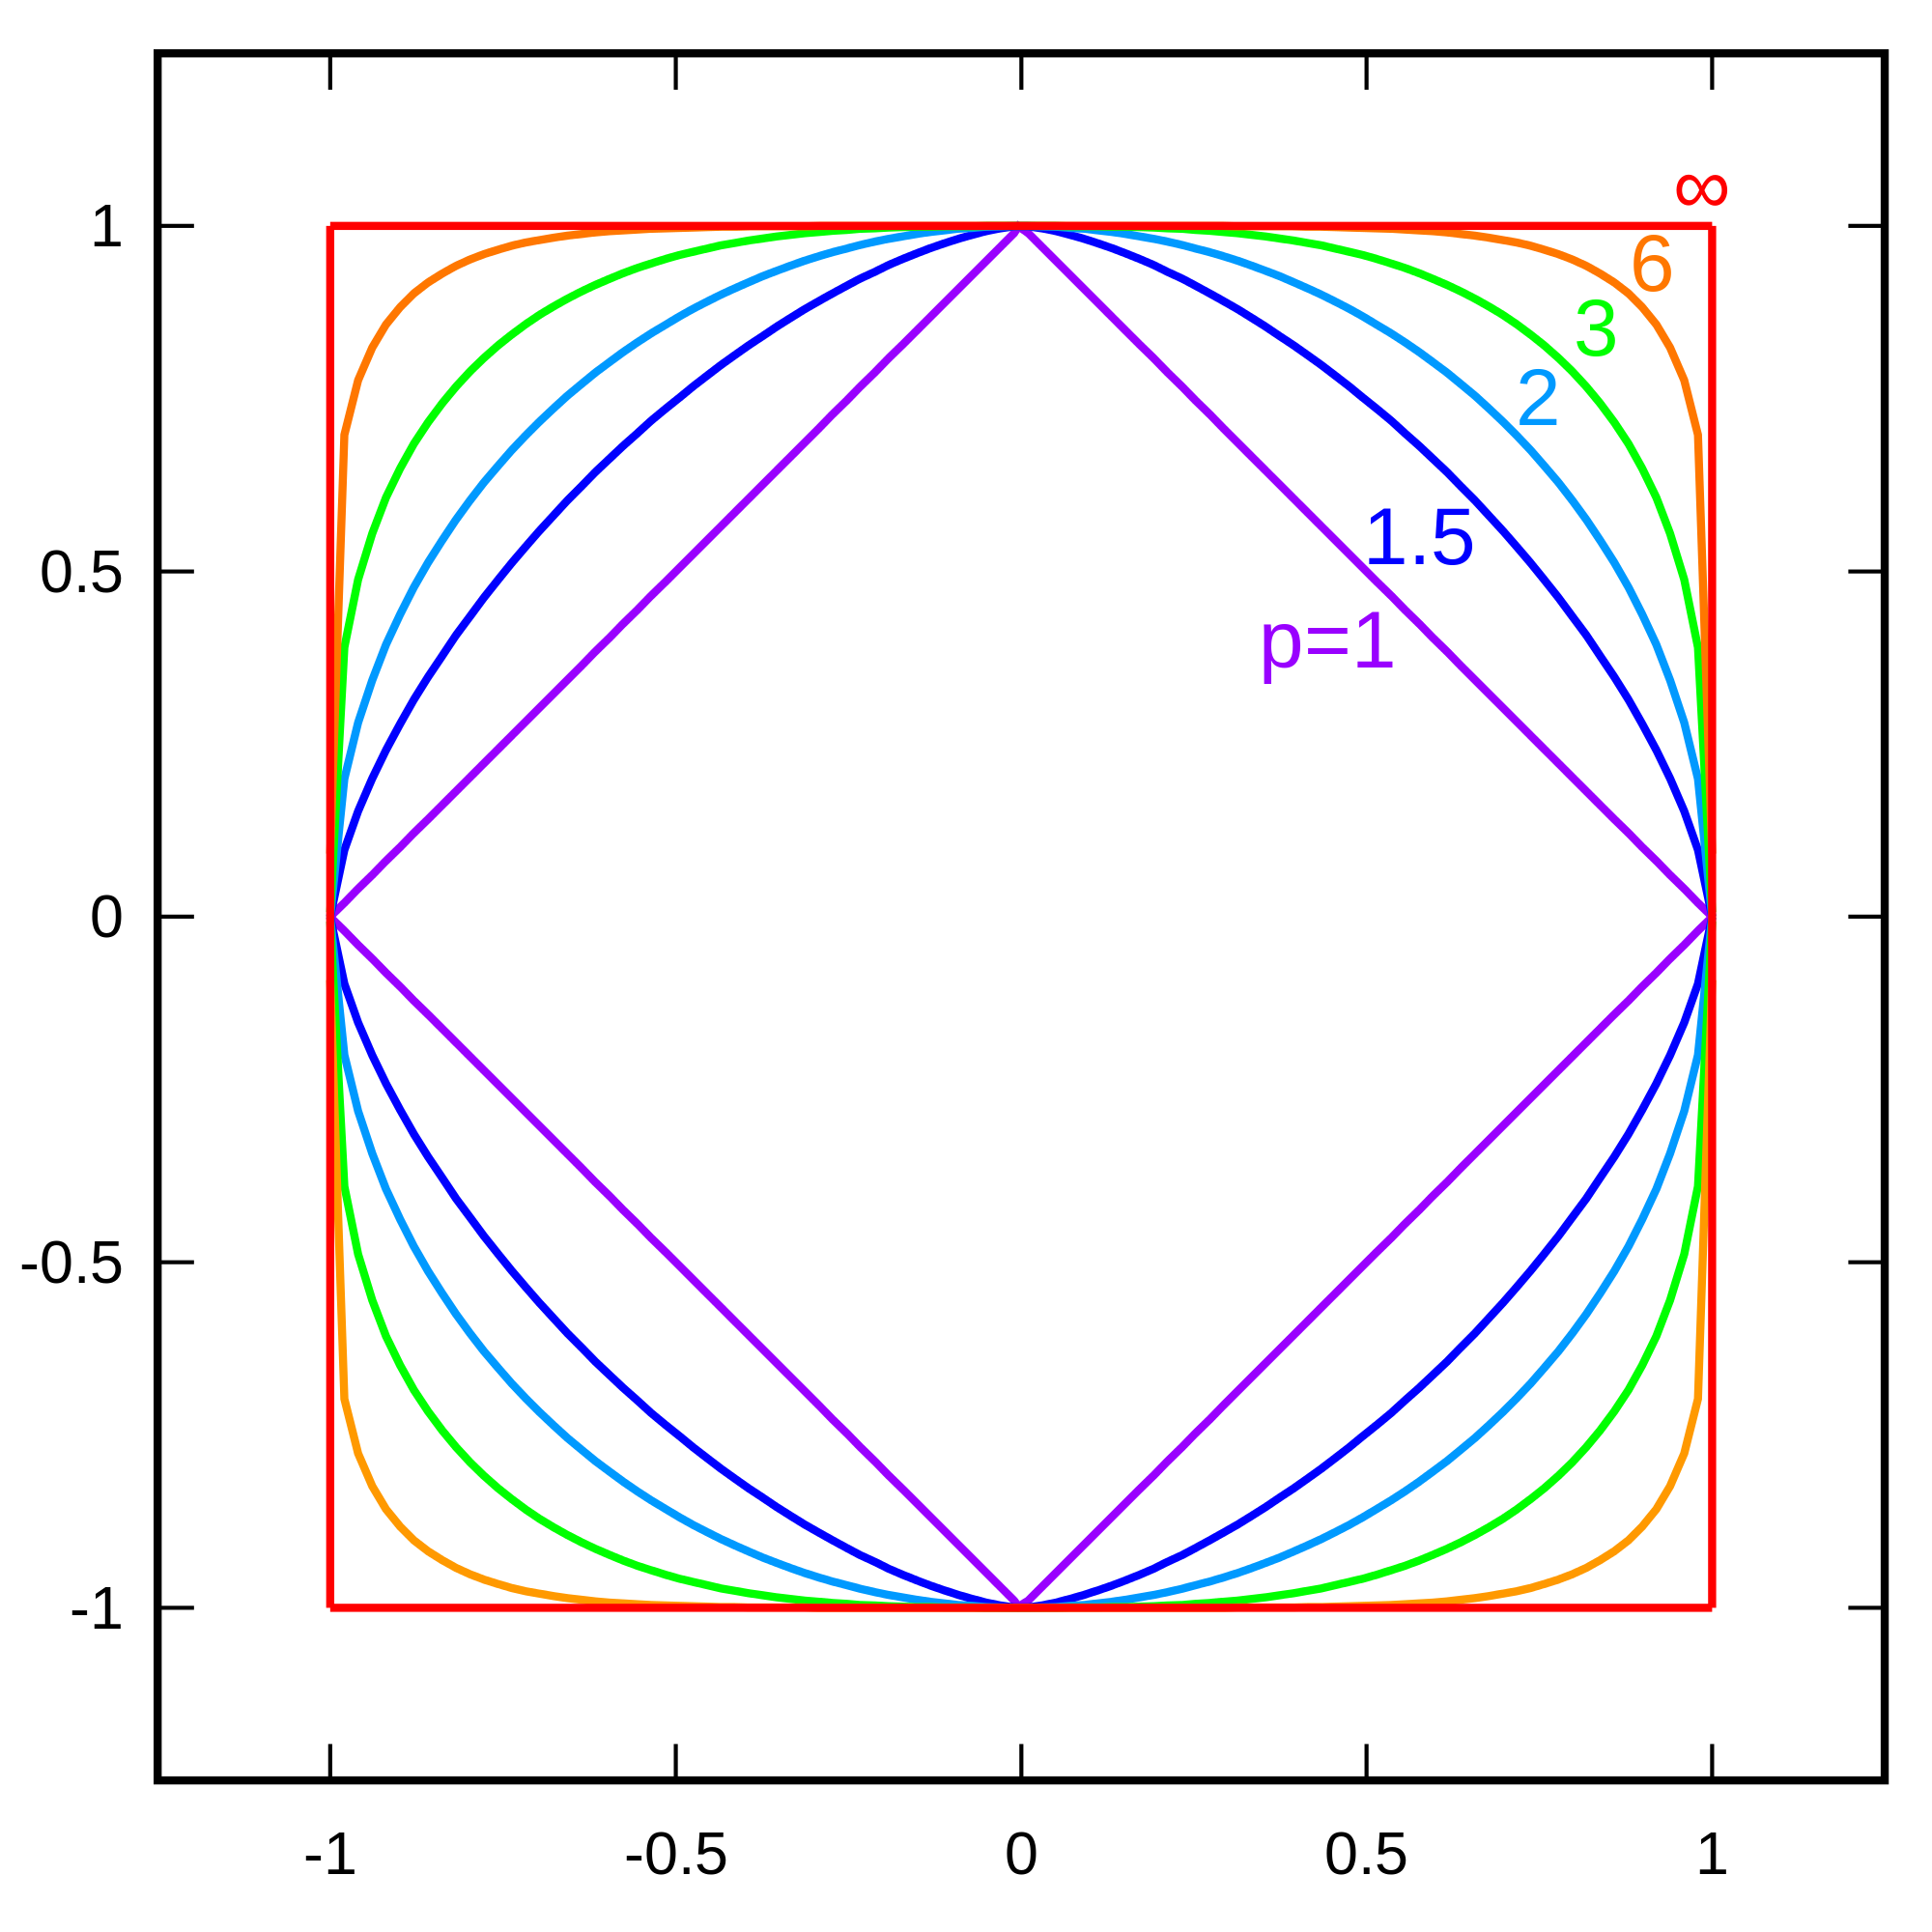
\includegraphics[width=0.5\textwidth]{figure_man/pnorm.png}
\end{center}

\framebreak 

Corresponding \textbf{matrix norm} (for $\Amat \in \R^{n \times n}$) is defined as
$$
\|\Amat\|_p := \sup_{\xv \not = \mathbf{0}}\left(\frac{\|\Amat \xv\|_p}{\|\xv\|_p}\right) =
  \sup_{\|\xv\|_p = 1} \left( \|\Amat\xv\|_p \right).
$$



\textbf{Examples} for matrix norms induced by vector norms:
\begin{itemize}
\item $\|\Amat\|_1 = \max_j\left(\sum_i |A_{ij}| \right) \quad$ (maximum absolute column sum norm)
  \begin{eqnarray*}
  \Amat = \begin{pmatrix*}[r]1 & -2 & -3 \\
  2 & 3 & -1\end{pmatrix*}\Rightarrow
  \|\Amat\|_1 &=& \max (\|A_1\|_1, \|A_2\|_1, \|A_3\|_1) \\
  &=& \max (3, 5, 4) = 5
  \end{eqnarray*}
\item $\|\Amat\|_2 = \left(\mbox{largest eigenvalue of } \Amat^\top\Amat \right)^{1/2} \quad$ (spectral norm)
\item $\|\Amat\|_\infty = \max_i\left(\sum_j |A_{ij}| \right) \quad$ (maximum absolute row sum norm)
\end{itemize}
\bigskip
Another common matrix norm is the \textbf{Frobenius norm} which can be interpreted as an extension of the Euclidean norm for vectors to matrices. It is defined as follows: 
$$
\|\Amat\|_F = \sqrt{\mbox{trace}(\Amat^\top\Amat)} = \sqrt{ \sum_i \sum_j A_{ij}^2}
$$
It is: $\quad \|\Amat\|_2 \leq \|\Amat\|_F$\\
\medskip
Most important to us is $\|.\| := \|.\|_2$

\framebreak

Intuition matrix norm:
\begin{itemize}
\item Longest possible \enquote{stretch} of a vector of length 1 when multiplied by $\Amat$.
\item For spectral norm: longest possible \enquote{stretch} in direction of the eigenvector of $\Amat^T\Amat$ (major axis of the ellipse) belonging to the largest absolute eigenvalue.
\end{itemize}

\begin{center}
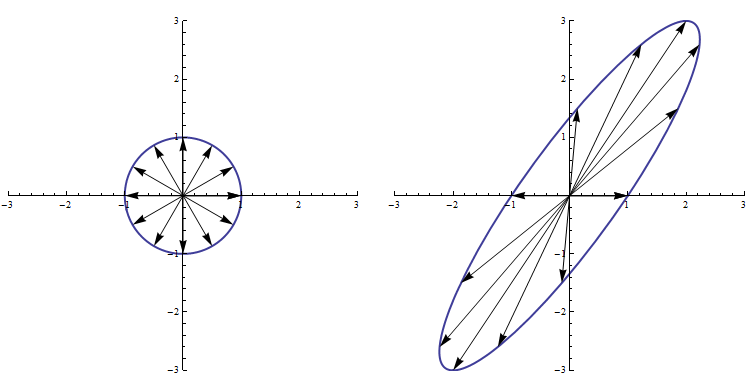
\includegraphics[width=0.5\textwidth]{figure_man/euklidischenorm.png}


\begin{footnotesize}
Left: Vectors of length 1. Right: Vectors after multiplication by $A$.
\end{footnotesize}
\end{center}

\framebreak

\begin{enumerate}
\item $ \|\Amat \xv\|_p \leq \|\Amat\|_p\|\xv\|_p,$ \\ 
  i.e., $\|\Amat\|_p$ is the smallest number to which this applies,
  because $\|\Amat\|_p \geq \frac{\|\Amat \xv\|_p}{\|\xv\|_p}$ for every $\xv \not= 0$.
  
\item $ \|\bm{AB}\|_p \leq \|\Amat\|_p \|\bm{B}\|_p$\\
  \vspace{0.2cm}
  \begin{footnotesize}
  \textbf{Proof:}
  Let $\xv$ be arbitrary with $\|\xv\|_p = 1$ Then
  $$
  \|\bm{ABx}\|_p \leq \|\Amat\|_p \|\bm{B}\xv\|_p \leq \|\Amat\|_p \|\bm{B}\|_p \|\xv\|_p = \|\Amat\|_p \|\bm{B}\|_p
  $$
  and thus 
  $$
  \|\bm{AB}\|_p = \sup_{\|\xv\|_p = 1} \|\bm{ABx}\|_p \leq \|\Amat\|_p \|\bm{B}\|_p
  $$
  
  \end{footnotesize}
  
\end{enumerate}


% \begin{eqnarray*}
% \|\mathbf{AB}\|_p &=& \sup \left( \frac{\|\mathbf{ABx}\|_p}{\|\xv\|_p} \right) \\
%   &=& \sup \left( \frac{\|\mathbf{ABx}\|_p}{\|\xv\|_p} \frac{\|\mathbf{Bx}\|_p}{\|\mathbf{Bx}\|_p} \right) \\
%   &=& \sup \left( \frac{\|\mathbf{ABx}\|_p}{\|\mathbf{Bx}\|_p} \frac{\|\mathbf{Bx}\|_p}{\|\xv\|_p} \right) \\
%   &\leq& \sup \left( \frac{\|\mathbf{ABx}\|_p}{\|\mathbf{Bx}\|_p} \right) \sup
%     \left(\frac{\|\mathbf{Bx}\|_p}{\|\xv\|_p} \right) \\
%   &=& \|\Amat\|_p\|\mathbf{B}\|_p.
% \end{eqnarray*}

\end{vbframe}



\endlecture
\end{document}
